\section{CFET(Complementary FET)構造}
CFET(Complementary Field-Effect Transistor)は、n型およびp型のトランジスタを垂直方向に積層した三次元デバイス構造であり、  
従来の平面配置(lateral arrangement)から垂直配置(vertical stacking)への構造転換を特徴とする。  
このアプローチにより、トランジスタ・セルが占有する平面面積を大幅に削減し、  
同一チップ面積あたりの集積度をFinFETやGAA構造を超えて向上させることが可能となる。

CFETでは、nFETとpFETが上下に積層され、それぞれ独立したゲートおよびソース/ドレイン構造を持つ。  
この垂直積層構造により、同一セル内で上下デバイスが相補的に動作するため、  
標準セル高さを縮小しながら論理駆動能力を維持できる。  
さらに、Backside Power Rail(BPR)技術との統合が容易であり、  
信号線と電源線の物理的分離によって配線抵抗および寄生結合を低減し、電源ノイズ耐性を向上させる。

GAA技術をベースとするCFETでは、上下のトランジスタを独立に電気的制御する必要があるため、  
チャネル層間のアイソレーション精度および熱干渉の抑制が設計上の要点となる。  
n型とp型デバイスが異なる移動度・発熱特性を有する場合、  
垂直方向の熱対称性(thermal symmetry)が支配因子となり、  
電流駆動能力および信頼性(NBTI/HCI耐性)に直接影響を及ぼす。

製造上の課題としては、垂直積層におけるソース/ドレインの選択的エピタキシャル成長、  
層間絶縁膜(Inter-Layer Dielectric; ILD)の平坦化精度、  
およびn/pトランジスタ間の電気的アイソレーション確保が挙げられる。  
特に、上部デバイス形成後に下部デバイス特性が劣化しないよう、  
プロセス全体の低温化($<400\,^{\circ}\mathrm{C}$)が不可欠である。  
このため、Selective EpitaxyやLow-Temperature ALDによるメタルゲート堆積など、  
熱負荷を最小限に抑えるプロセス技術が開発されている。

CFETは、GAAを超えて「論理対称性と物理空間効率の両立」を実現する究極の三次元CMOSアーキテクチャである。  
現在、IMEC、Intel、Samsungなどの主要研究機関・メーカーが試作段階に到達しており、  
1\,nmクラス以降のロジックデバイスにおける有力な主流候補と位置付けられている。  
次章では、こうした三次元構造を支える配線および電源インテグレーション技術(BEOLおよびBPR)について論じる。

\begin{table}[t]
  \centering
  \caption{CFET(Complementary FET)構造設計パラメータ}
  \label{tab:cfet_stack}
  \begin{tabular}{lccc}
    \toprule
    項目 & 記号 & 代表値 & 備考 \\
    \midrule
    n/p積層距離 & $d_{np}$ & 20–30\,nm & 熱干渉最小化に設計 \\
    上部チャネル厚 & $T_p$ & 5–7\,nm & pFET層 \\
    下部チャネル厚 & $T_n$ & 5–7\,nm & nFET層 \\
    絶縁層厚 & $T_\mathrm{ILD}$ & 10\,nm & 熱・電気分離層 \\
    BPR金属厚 & $T_\mathrm{BPR}$ & 100–150\,nm & 電源層再配置 \\
    電源分離効率 & $\eta_\mathrm{BPR}$ & $>$90\% & IRドロップ低減効果 \\
    面積削減率 & $A_\mathrm{red}$ & 35–40\% & FinFET比 \\
    \bottomrule
  \end{tabular}
\end{table}

% =====================================================
% Fig. 7 : CFET(Complementary FET)垂直積層構造 断面図
% =====================================================
\begin{figure}[t]
  \centering
  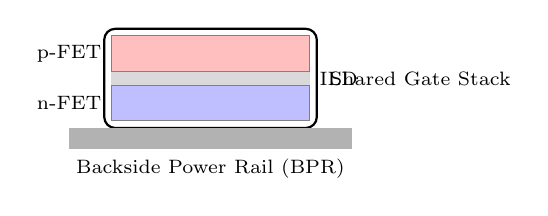
\begin{tikzpicture}[scale=0.9, every node/.style={font=\scriptsize}]
    % bottom n-FET
    \fill[blue!25] (0.6,0.4) rectangle (3.4,0.9);
    \draw[black!50] (0.6,0.4) rectangle (3.4,0.9);
    \node[left] at (0.6,0.65) {n-FET};

    % isolation (ILD)
    \fill[gray!30] (0.6,0.9) rectangle (3.4,1.1);
    \node[right] at (3.4,1.0) {ILD};

    % top p-FET
    \fill[red!25] (0.6,1.1) rectangle (3.4,1.6);
    \draw[black!50] (0.6,1.1) rectangle (3.4,1.6);
    \node[left] at (0.6,1.35) {p-FET};

    % gate stack
    \draw[thick,rounded corners] (0.5,0.3) rectangle (3.5,1.7);
    \node[right] at (3.55,1.0) {Shared Gate Stack};

    % backside power rail (BPR)
    \fill[gray!60] (0,0) rectangle (4,0.3);
    \node[below] at (2,0) {Backside Power Rail (BPR)};
  \end{tikzpicture}

  \caption{CFET構造の垂直積層模式図(n/pスタックおよびBPRを示す)\\
  \footnotesize Schematic vertical stack of CFET showing n/p layers and backside power rail.}
  \label{fig:cfet_cross}
\end{figure}

